\documentclass[twocolumn]{../common/aa}
%\documentclass[referee]{aa}

\usepackage{graphicx}
\usepackage{amsmath,amsfonts,amssymb}
\usepackage{txfonts}
\usepackage{color}
\usepackage{natbib}
\usepackage{float}
%\usepackage{stfloats}
\usepackage{dblfloatfix}
\usepackage{afterpage}
\usepackage{ifthen}
\usepackage[morefloats=12]{morefloats}
\usepackage{placeins}
\usepackage{multicol}
\bibpunct{(}{)}{;}{a}{}{,}
\usepackage[switch]{lineno}
\definecolor{linkcolor}{rgb}{0.6,0,0}
\definecolor{citecolor}{rgb}{0,0,0.75}
\definecolor{urlcolor}{rgb}{0.12,0.46,0.7}
\usepackage[breaklinks, colorlinks, urlcolor=urlcolor,
    linkcolor=linkcolor,citecolor=citecolor,pdfencoding=auto]{hyperref}
\hypersetup{linktocpage}
\usepackage{bold-extra}
\usepackage{xcolor}

%\usepackage[grid,
%  gridcolor=red!20,
%  subgridcolor=green!20,
%  gridunit=cm]{eso-pic}
%

%Planck style file, to be used with A&A style to produce Planck papers for publication.
%
% version 28 September 2010 --- useful macros --- CRL
% version 17 October 2010   --- first cut at important instrument values, from Daniele Mennella and
%                               Francois Bouchet, 13 October 2010 --- CRL
% version 18 October 2010   --- LFI FWHM changed to one value per feed, rather than M & S separately
%                               LFI FWHM uncertainties added for individual feeds.  Corrections made
%                               to LFI values. --- Andrea Zacchei
% version 24 October 2010   --- added to and corrected definitions.  No changes made to instrument
%                               quantities. --- CRL 
% version 31 October 2010   --- added definition of \muKHz. --- CRL
%
% version 15 November 2010  --- fixed conflict with aa.cls in definition of \endtable
%                               by naming the command below "\endPlancktable".  See section
%                               13.16 of the Style Guide.
%
% version 06 December 2010  --- Set up names with and without units.
%                               Add \allearlypapers command to ensure that all early papers are
%                               included in the reference list.
%                               Define macro for the name of the 4He JT cooler.
%
% version 07 December 2010  --- removed extraneous "planck2011-1.2" entry in \allearlypapers
%
% version 12 December 2010  --- added \endPlancktablewide command to set tablenotes to the full
%                               page width in the \begin{table*}...\end{table*} environment when
%                               the ``twocolumn'' option is specified in the \documentclass command.
%                               (It would be more elegant to extract the appropriate width from the
%                               aa.cls system at the time of execution, but that is buried more
%                               deeply in the system than I investigated.)
%
% version 05 January 2011   --- added unit \MJysr.  HFI performance values updated per FRB email
%                               01/05/2011 02:38-0800, and Brendan Crill email 01/05/2011 18:08 -0800.
%
% version 06 January 2011   --- changed \scriptscriptstyle primes to \scriptstyle, to better match the
%                               tx fonts used by A&A.
%
% version 07 January 2011   --- modified \allearlypapers to correspond with final early paper list.  
%                               Fixed 545 GHz center frequency.
%
% version 07 January 2011b  --- changed LFI white-noise sensitivity numbers to correct problem with units
%
% version 05 July 2011      --- added \Msol and \Lsol to get the symbols for solar mass and luminosity.
%                               Deleted previous definitions of \solar and \sol, which were equivalent
%                               to the new \Msol.
%
% version 16 August 2011    --- changed comments on \endPlancktable and \endPlancktablewide for clarity
%
% version 11 September 2011 --- changed definition of \tablenote to make footnote labels italic, as per A\&A
%
% version 26 April 2011     --- changed definition of \Planck to agree with what is said in the Style Guide (!)
%
% version 04 Dec 2013       --- included 2013 results references
%
% version 17 Jan 2014       --- included fix to bibtex file v4.3, i.e. \providecommand{\sorthelp}[1]{}
%
% version 26 Jul 2014       --- fixed incompatibility problem with aa.cls v8.0 and v8.2.  v8.2 should now be used
%                               for all Planck papers.
%                           --- fixed problem in definition of "\all2013resultspapers" that introduced a blanck
%                               into the reference to p06b.
%                           --- removed all the parameter definition stuff at the end.  We weren't using it, and
%                               it took up a lot of space.
%
% version 28 Jan 2015       --- added "\alltwentyfiftennresultspapers" and corrected "\all2013resultspapers" to
%                               "\all20thirteenresultspapers",
%
% Usage:  after the \documentclass[traditabstract]{aa} command in the La\TeX\ input file,
%         add this command:      \input Planck.tex


\def\setsymbol#1#2{\expandafter\def\csname #1\endcsname{#2}}
\def\getsymbol#1{\csname #1\endcsname}

%-----------------------------------------------------------------------
% Planck
%-----------------------------------------------------------------------
\def\Planck{\textit{Planck}}

%-----------------------------------------------------------------------
% The Planck Helium-4 JT cooler
%-----------------------------------------------------------------------
\def\HeJT{$^4$He-JT}

%-----------------------------------------------------------------------
% To include all Planck Early Results papers in the reference lists
%-----------------------------------------------------------------------
\def\allearlypapers{\nocite{planck2011-1.1, planck2011-1.3, planck2011-1.4, planck2011-1.5, planck2011-1.6, planck2011-1.7, planck2011-1.10, planck2011-1.10sup, planck2011-5.1a, planck2011-5.1b, planck2011-5.2a, planck2011-5.2b, planck2011-5.2c, planck2011-6.1, planck2011-6.2, planck2011-6.3a, planck2011-6.4a, planck2011-6.4b, planck2011-6.6, planck2011-7.0, planck2011-7.2, planck2011-7.3, planck2011-7.7a, planck2011-7.7b, planck2011-7.12, planck2011-7.13}}

%-----------------------------------------------------------------------
% To include all Planck 2013 Results papers in the reference lists
%-----------------------------------------------------------------------
\def\alltwentythirteenresultspapers{\nocite{planck2013-p01, planck2013-p02, planck2013-p02a, planck2013-p02d, planck2013-p02b, planck2013-p03, planck2013-p03c, planck2013-p03f, planck2013-p03d, planck2013-p03e, planck2013-p01a, planck2013-p06, planck2013-p03a, planck2013-pip88, planck2013-p08, planck2013-p11, planck2013-p12, planck2013-p13, planck2013-p14, planck2013-p15, planck2013-p05b, planck2013-p17, planck2013-p09, planck2013-p09a, planck2013-p20, planck2013-p19, planck2013-pipaberration, planck2013-p05, planck2013-p05a, planck2013-pip56, planck2013-p06b, planck2013-p01a}}

%-----------------------------------------------------------------------
% To include all Planck 2015 Results papers in the reference lists
%-----------------------------------------------------------------------
\def\alltwentyfifteenresultspapers{\nocite{planck2014-a01, planck2014-a03, planck2014-a04, planck2014-a05, planck2014-a06, planck2014-a07, planck2014-a08, planck2014-a09, planck2014-a11, planck2014-a12, planck2014-a13, planck2014-a14, planck2014-a15, planck2014-a16, planck2014-a17, planck2014-a18, planck2014-a19, planck2014-a20, planck2014-a22, planck2014-a24, planck2014-a26, planck2014-a28, planck2014-a29, planck2014-a30, planck2014-a31, planck2014-a35, planck2014-a36, planck2014-a37, planck2014-ES}}

%-----------------------------------------------------------------------
% Tables
%-----------------------------------------------------------------------
\newbox\tablebox    \newdimen\tablewidth
\def\leaderfil{\leaders\hbox to 5pt{\hss.\hss}\hfil}
%
% use the following definition of \endPlancktable for ApJ style notes to tables, set to the 
%         width of the table
% \def\endPlancktable{\tablewidth=\wd\tablebox 
%
% use the following definitions of \endPlancktable and \endPlancktablewide for A&A style notes 
% set to one-column  or full-page width, respectively
\def\endPlancktable{\tablewidth=\columnwidth 
    $$\hss\copy\tablebox\hss$$
    \vskip-\lastskip\vskip -2pt}
\def\endPlancktablewide{\tablewidth=\textwidth 
    $$\hss\copy\tablebox\hss$$
    \vskip-\lastskip\vskip -2pt}
\def\tablenote#1 #2\par{\begingroup \parindent=0.8em
    \abovedisplayshortskip=0pt\belowdisplayshortskip=0pt
    \noindent
    $$\hss\vbox{\hsize\tablewidth \hangindent=\parindent \hangafter=1 \noindent
    \hbox to \parindent{$^#1$\hss}\strut#2\strut\par}\hss$$
    \endgroup}
\def\doubleline{\vskip 3pt\hrule \vskip 1.5pt \hrule \vskip 5pt}

%-----------------------------------------------------------------------
% useful macros
%-----------------------------------------------------------------------
%
\def\L2{\ifmmode L_2\else $L_2$\fi}
%
\def\dtt{\Delta T/T}
\def\DeltaT{\ifmmode \Delta T\else $\Delta T$\fi}
\def\deltat{\ifmmode \Delta t\else $\Delta t$\fi}
\def\fknee{\ifmmode f_{\rm knee}\else $f_{\rm knee}$\fi}
\def\Fmax{\ifmmode F_{\rm max}\else $F_{\rm max}$\fi}
%
\def\solar{\ifmmode{\rm M}_{\mathord\odot}\else${\rm M}_{\mathord\odot}$\fi}
\def\Msolar{\ifmmode{\rm M}_{\mathord\odot}\else${\rm M}_{\mathord\odot}$\fi}
\def\Lsolar{\ifmmode{\rm L}_{\mathord\odot}\else${\rm L}_{\mathord\odot}$\fi}
%
\def\inv{\ifmmode^{-1}\else$^{-1}$\fi}
\def\mo{\ifmmode^{-1}\else$^{-1}$\fi}
\def\sup#1{\ifmmode ^{\rm #1}\else $^{\rm #1}$\fi}
\def\expo#1{\ifmmode \times 10^{#1}\else $\times 10^{#1}$\fi}
%
\def\,{\thinspace}
\def\lsim{\mathrel{\raise .4ex\hbox{\rlap{$<$}\lower 1.2ex\hbox{$\sim$}}}}
\def\gsim{\mathrel{\raise .4ex\hbox{\rlap{$>$}\lower 1.2ex\hbox{$\sim$}}}}
\let\lea=\lsim
\let\gea=\gsim
\def\simprop{\mathrel{\raise .4ex\hbox{\rlap{$\propto$}\lower 1.2ex\hbox{$\sim$}}}}
%
\def\deg{\ifmmode^\circ\else$^\circ$\fi}
\def\pdeg{\ifmmode $\setbox0=\hbox{$^{\circ}$}\rlap{\hskip.11\wd0 .}$^{\circ}
          \else \setbox0=\hbox{$^{\circ}$}\rlap{\hskip.11\wd0 .}$^{\circ}$\fi}
\def\arcs{\ifmmode {^{\scriptstyle\prime\prime}}
          \else $^{\scriptstyle\prime\prime}$\fi}
\def\arcm{\ifmmode {^{\scriptstyle\prime}}
          \else $^{\scriptstyle\prime}$\fi}
\newdimen\sa  \newdimen\sb
\def\parcs{\sa=.07em \sb=.03em
     \ifmmode \hbox{\rlap{.}}^{\scriptstyle\prime\kern -\sb\prime}\hbox{\kern -\sa}
     \else \rlap{.}$^{\scriptstyle\prime\kern -\sb\prime}$\kern -\sa\fi}
\def\parcm{\sa=.08em \sb=.03em
     \ifmmode \hbox{\rlap{.}\kern\sa}^{\scriptstyle\prime}\hbox{\kern-\sb}
     \else \rlap{.}\kern\sa$^{\scriptstyle\prime}$\kern-\sb\fi}
%
\def\ra[#1 #2 #3.#4]{#1\sup{h}#2\sup{m}#3\sup{s}\llap.#4}
\def\dec[#1 #2 #3.#4]{#1\deg#2\arcm#3\arcs\llap.#4}
\def\deco[#1 #2 #3]{#1\deg#2\arcm#3\arcs}
\def\rra[#1 #2]{#1\sup{h}#2\sup{m}}
%
\def\page{\vfill\eject}
\def\dots{\relax\ifmmode \ldots\else $\ldots$\fi}
%
%-----------------------------------------------------------------------
% units
%-----------------------------------------------------------------------
%
\def\WHzsr{\ifmmode $W\,Hz\mo\,sr\mo$\else W\,Hz\mo\,sr\mo\fi}
\def\mHz{\ifmmode $\,mHz$\else \,mHz\fi}
\def\GHz{\ifmmode $\,GHz$\else \,GHz\fi}
\def\mKs{\ifmmode $\,mK\,s$^{1/2}\else \,mK\,s$^{1/2}$\fi}
\def\muKs{\ifmmode \,\mu$K\,s$^{1/2}\else \,$\mu$K\,s$^{1/2}$\fi}
\def\muKRJs{\ifmmode \,\mu$K$_{\rm RJ}$\,s$^{1/2}\else \,$\mu$K$_{\rm RJ}$\,s$^{1/2}$\fi}
\def\muKHz{\ifmmode \,\mu$K\,Hz$^{-1/2}\else \,$\mu$K\,Hz$^{-1/2}$\fi}
\def\MJysr{\ifmmode \,$MJy\,sr\mo$\else \,MJy\,sr\mo\fi}
\def\MJysrmK{\ifmmode \,$MJy\,sr\mo$\,mK$_{\rm CMB}\mo\else \,MJy\,sr\mo\,mK$_{\rm CMB}\mo$\fi}
\def\microns{\ifmmode \,\mu$m$\else \,$\mu$m\fi}
\def\micron{\microns}
\def\muK{\ifmmode \,\mu$K$\else \,$\mu$\hbox{K}\fi}
\def\microK{\ifmmode \,\mu$K$\else \,$\mu$\hbox{K}\fi}
\def\muW{\ifmmode \,\mu$W$\else \,$\mu$\hbox{W}\fi}
\def\kms{\ifmmode $\,km\,s$^{-1}\else \,km\,s$^{-1}$\fi}
\def\kmsMpc{\ifmmode $\,\kms\,Mpc\mo$\else \,\kms\,Mpc\mo\fi}
%
%
%----------------------------------------------------------------------
% set up machinery to list Planck papers in roman numeral order.
%----------------------------------------------------------------------

\providecommand{\sorthelp}[1]{}


\def\WMAP{\emph{WMAP}}
\def\WMAPnine{\emph{WMAP9}}
\def\COBE{\emph{COBE}}
\def\wmap{\emph{WMAP}}
\def\planck{\emph{Planck}}
\def\Planck{\emph{Planck}}
\def\LCDM{$\Lambda$CDM}
\def\ffp{FFP6}
\def\unionmask{U73}
\def\nside{N_{\mathrm{side}}}

\def\healpix{\texttt{HEALPix}}
\def\commander{\texttt{Commander}}
\def\commanderone{\texttt{Commander1}}
\def\commandertwo{\texttt{Commander2}}
\def\commanderthree{\texttt{Commander3}}
\def\ruler{\texttt{Ruler}}
\def\comrul{\texttt{Commander-Ruler}}
\def\CR{\texttt{C-R}}
\def\nilc{\texttt{NILC}}
\def\gnilc{\texttt{GNILC}}
\def\sevem{\texttt{SEVEM}}
\def\smica{\texttt{SMICA}}
\def\CamSpec{\texttt{CamSpec}}
\def\Plik{\texttt{Plik}}
\def\XFaster{\texttt{XFaster}}
\def\sroll2{\texttt{SRoll2}}

\renewcommand{\d}[0]{\vec{d}}
\renewcommand{\t}[0]{\vec{t}}
\newcommand{\A}[0]{\mathrm{A}}
\newcommand{\B}[0]{\mathrm{B}}
\newcommand{\Y}[0]{\tens{Y}}
\newcommand{\n}[0]{\vec{n}}
\newcommand{\red}[0]{\color{red}}
\newcommand{\green}[0]{\color{green}}
\newcommand{\s}[0]{\vec{s}}
\renewcommand{\a}[0]{\vec{a}}
\newcommand{\m}[0]{\vec{m}}
\newcommand{\f}[0]{\vec{f}}
\newcommand{\F}[0]{\tens{F}}
\newcommand{\T}[0]{\tens{T}}
\newcommand{\Cp}[0]{\tens{C}}
\renewcommand{\L}[0]{\tens{L}}
\newcommand{\g}[0]{\vec{g}}
\newcommand{\N}[0]{\tens{N}}
\newcommand{\M}[0]{\tens{M}}
\newcommand{\iN}[0]{\tens{N}^{-1}}
\newcommand{\iM}[0]{\tens{M}^{-1}}
\newcommand{\w}[0]{\vec{w}}
\renewcommand{\S}[0]{\tens{S}}
\renewcommand{\r}[0]{\vec{r}}
\renewcommand{\u}[0]{\vec{u}}
\newcommand{\q}[0]{\vec{q}}
\renewcommand{\v}[0]{\vec{v}}
\renewcommand{\P}[0]{\tens{P}}
\newcommand{\dt}[0]{d_t}
\newcommand{\di}[0]{d_i}
\newcommand{\nt}[0]{n_t}
\newcommand{\st}[0]{s_t}
\newcommand{\mt}[0]{m_t}
\newcommand{\ft}[0]{f_t}
\newcommand{\Te}[0]{T_{\rm e}}
\newcommand{\EM}[0]{\rm EM}
\newcommand{\mathsc}[1]{{\normalfont\textsc{#1}}}
\newcommand{\hi}{\ensuremath{\mathsc {Hi}}}
\newcommand{\bpbold}{\bfseries{\scshape{BeyondPlanck}}}
\newcommand{\BP}{\textsc{BeyondPlanck}}
\newcommand{\bp}{\textsc{BeyondPlanck}}
\newcommand{\cosmoglobe}{\textsc{Cosmoglobe}}
\newcommand{\Cosmoglobe}{\textsc{Cosmoglobe}}
\newcommand{\lfi}[0]{LFI}
\newcommand{\hfi}[0]{HFI}
\newcommand{\npipe}[0]{\texttt{NPIPE}}
\newcommand{\K}[0]{\textit K}
\newcommand{\Ka}[0]{\textit{Ka}}
\newcommand{\Q}[0]{\textit Q}
\newcommand{\V}[0]{\textit V}
\newcommand{\W}[0]{\textit W}
\newcommand{\e}{\mathrm e}
\newcommand{\cvar}{\ensuremath{c(\vartheta, \varphi, \psi)}}


\def\bC{\tens{C}}
\def\ba{\vec{a}}
\def\ncha{N_\mathrm{cha}}
\def\nfg{N_\mathrm{fg}}

\newcommand{\data}{\vec d}
\newcommand{\ncorr}{\vec n_\mathrm{corr}}
\newcommand{\Dbp}{\Delta_\mathrm{bp}}

%\modulolinenumbers[5]
%\linenumbers

\newcommand{\includegraphicsdpi}[3]{
    \pdfimageresolution=#1  % Change the dpi of images
    \includegraphics[#2]{#3}
    \pdfimageresolution=72  % Change it back to the default
}

\renewcommand{\topfraction}{1.0}	% max fraction of floats at top
    \renewcommand{\bottomfraction}{1.0}	% max fraction of floats at bottom
    %   Parameters for TEXT pages (not float pages):
    \setcounter{topnumber}{2}
    \setcounter{bottomnumber}{2}
    \setcounter{totalnumber}{4}     % 2 may work better
    \setcounter{dbltopnumber}{2}    % for 2-column pages
    \renewcommand{\dbltopfraction}{0.9}	% fit big float above 2-col. text
    \renewcommand{\textfraction}{0.04}	% allow minimal text w. figs
    %   Parameters for FLOAT pages (not text pages):
    \renewcommand{\floatpagefraction}{0.9}	% require fuller float pages
	% N.B.: floatpagefraction MUST be less than topfraction !!
    \renewcommand{\dblfloatpagefraction}{0.9}	% require fuller float pages

\def\adj{^{\dagger}}
\def\tp{^{\rm T}}
\def\inv{^{-1}}
\def\lm{{\ell m}}

\begin{document}

\title{\bfseries{\Cosmoglobe: Towards likelihood-free CMB cosmological\\ parameter estimation with end-to-end error propagation}}
%This author list corresponds to \title{Author list for L04\_CMB\_Foregrounds\_Extraction}
%Prepared by M. Lopez-Caniego (Marcos.Lopez.Caniego@sciops.esa.int), ESAC/ESA
%This version is from Thu Jul 12 18:11:48 2018 CET
%\subtitle{There are 152 co-authors in this list}
\newcommand{\oslo}[0]{1}
\newcommand{\iiabangalore}[0]{2}

\author{\small
D.~J.~Watts\inst{\ref{uio}}\thanks{Corresponding author: D.~J.~Watts; \url{duncanwa@astro.uio.no}}
\and
A.~Basyrov\inst{\ref{uio}}
\and
H.~T.~Ihle\inst{\ref{uio}}
\and
S.~Paradiso\inst{\ref{waterloo}}
\and
F.~Rahman\inst{\ref{iiabangalore}}
\and
H.~Thommesen\inst{\ref{uio}}
\and
M.~Bersanelli\inst{\ref{milan}}
\and
L.~A.~Bianchi\inst{\ref{milan}}
\and
M.~Brilenkov\inst{\ref{uio}}
\and
L.~P.~L.~Colombo\inst{\ref{milan}}
\and
H.~K.~Eriksen\inst{\ref{uio}}
\and
J.~R.~Eskilt\inst{\ref{uio},\ref{imperial}}
\and
K.~S.~F.~Fornazier\inst{\ref{saopaulo}}
\and
C.~Franceschet\inst{\ref{milan}}
\and
U.~Fuskeland\inst{\ref{uio}}
\and
M.~Galloway\inst{\ref{uio}}
\and
E.~Gjerl\o w\inst{\ref{uio}}
\and
B.~Hensley\inst{\ref{princeton}}
\and
L.~T.~Hergt\inst{\ref{ubc}}
\and
D.~Herman\inst{\ref{uio}}
\and
G.~A.~Hoerning\inst{\ref{saopaulo}}
\and
K.~Lee\inst{\ref{uio}}
\and
J.~G.~S.~Lunde\inst{\ref{uio}}
\and
A.~Marins\inst{\ref{saopaulo},\ref{ustofc}}
\and
S.~K.~Nerval\inst{\ref{dunlap1},\ref{dunlap2}}
\and
S.~K.~Patel\inst{\ref{iit_bhu}}
\and
M.~Regnier\inst{\ref{apc}}
\and
M.~San\inst{\ref{uio}}
\and
S.~Sanyal\inst{\ref{iit_bhu}}
\and
N.-O.~Stutzer\inst{\ref{uio}}
\and
A.~Verma\inst{\ref{iit_bhu}}
\and
I.~K.~Wehus\inst{\ref{uio}}
\and
Y.~Zhou\inst{\ref{berkeley}}
}
\institute{\small
Institute of Theoretical Astrophysics, University of Oslo, Blindern, Oslo, Norway\label{uio}
\and
Waterloo Centre for Astrophysics, University of Waterloo, Waterloo, ON N2L 3G1, Canada\label{waterloo}
\and
Indian Institute of Astrophysics, Koramangala II Block, Bangalore, 560034, India\label{iiabangalore}
\and
Dipartimento di Fisica, Università degli Studi di Milano, Via Celoria, 16, Milano, Italy\label{milan}
\and
Imperial Centre for Inference and Cosmology, Department of Physics, Imperial College London, Blackett Laboratory, Prince Consort Road, London SW7 2AZ, United Kingdom\label{imperial}
\and
Instituto de Física, Universidade de São Paulo - C.P. 66318, CEP: 05315-970, São Paulo, Brazil\label{saopaulo}
\and
Department of Astrophysical Sciences, Princeton University, 4 Ivy Lane, Princeton, NJ 08540\label{princeton}
\and
Department of Physics and Astronomy, University of British Columbia, 6224 Agricultural Road, Vancouver BC, V6T1Z1, Canada\label{ubc}
\and
Department of Astronomy,  University of Science and Technology of China, Hefei, China\label{ustofc}
\and
David A. Dunlap Department of Astronomy \& Astrophysics, University of Toronto, 50 St. George Street, Toronto, ON M5S 3H4, Canada\label{dunlap1}
\and
Dunlap Institute for Astronomy \& Astrophysics, University of Toronto, 50 St. George Street, Toronto, ON M5S 3H4, Canada\label{dunlap2}
\and
Department of Physics, Indian Institute of Technology (BHU), Varanasi - 221005, India\label{iit_bhu}
\and
Laboratoire Astroparticule et Cosmologie (APC), Université Paris-Cité, Paris, France\label{apc}
\and
Department of Physics, UC Berkeley\label{berkeley}
}

 %\author{V.~Arsenijevic\inst{\ref{inst1}}\and S.~Fabbro\inst{\ref{inst2}}\and
%A.~M.~Mour\~ao\inst{\ref{inst3}}\and A.~J.~Rica da Silva\inst{\ref{inst1}}}
%
%\institute{Multidisciplinar de Astrof\'{\i}sica, IST, Avenida Rovisco Pais, 1049
%Lisbon, Portugal\email{...}\label{inst1} \and < Multidisciplinar de Astrof\'{\i}sica, IST, Avenida Rovisco Pais, 1049 Lisbon, Portugal\email{...}\label{inst2}
%\and
%Multidisciplinar de Astrof\'{\i}sica, IST, Avenida Rovisco Pais, 1049
%Lisbon, Portugal\email{...}\label{inst3}
%} 

%\authorrunning{From BeyondPlanck to Cosmoglobe}
\authorrunning{Eskilt et al.}
\titlerunning{CMB parameter estimation}

\abstract{
  We implement support for likelihood-free cosmological parameter estimation algorithm, as originally proposed by Racine et al.\ (2016), in the world's first end-to-end Bayesian CMB Gibbs sampler called \commander, and quantify its computational efficiency and cost. For a semi-realistic simulation with noise levels similar to \Planck\ LFI 70\,GHz, a maximum multipole of $\ell_{\mathrm{max}}=1300$, and an accepted sky fraction of $f_{\mathrm{sky}}=0.85$, we find that more than 5000 Conjugate Gradient iterations are required to achieve sufficient CMB map accuracy, and that the typical Markov chain correlation length is $\sim$\,100 samples. The net effective cost per independent sample is $\sim$\,5000\,CPU-hrs, which --- when integrated into a full end-to-end Bayesian pipeline --- is to be compared with the sum of all lower-level processing costs. As a relevant example, processing all \Planck\ LFI and \WMAP\ channels within the \cosmoglobe\ Data Release 1 pipeline costs 812\,CPU-hrs, and the addition of the new parameter estimation step discussed here will therefore increase the overall analysis cost of that particular data set by a factor of six. Thus, although technically possible to run already in its current state, future work should aim to reduce the effective cost per independent sample by at least one order of magnitude to avoid excessive runtimes; we argue that this is possible through improved multi-grid preconditioners and/or derivative-based Markov chain sampling schemes. At the same time, we also note that both the Conjugate Gradient mapmaking cost and the Markov chain correlation length depend strongly on the signal-to-noise ratio of the data in question, and next-generation CMB $B$-mode satellite polarization measurements generally have a much lower signal-to-noise ratio than \Planck\ and \WMAP's temperature constraints. On the one hand, this work demonstrates the computational feasiblity of true Bayesian cosmological parameter estimation with end-to-end error propagation for high-precision CMB experiments without likelihood approximations; on the other hand, it also highlights the need for additional optimizations before it is justified for full production-level analysis. 
}

\keywords{ISM: general -- Cosmology: observations, polarization,
    cosmic microwave background, diffuse radiation -- Galaxy:
    general}

\maketitle

%\hypersetup{linkcolor=black}
\tableofcontents
%\hypersetup{linkcolor=red} 




\section{Introduction}
\label{sec:introduction}

High-precision cosmic microwave background (CMB) measurements provide today the strongest constraints on a wide range of key cosmological parameters \citep[e.g.,][]{planck2016-l06}. Traditionally, these constraints are derived by first compressing the information contained in the high-dimensional raw time-ordered data into pixelized sky maps and angular power spectra \citep[e.g.,][]{bennett2012,planck2016-l02,planck2016-l03}, and this compressed dataset is typically summarized in terms of a low-dimensional power spectrum-based likelihood from which cosmological parameters are derived through Markov Chain Monte Carlo sampling \citep{cosmomc,planck2016-l05}.

The key element in this pipeline procedure is the likelihood function, $\mathcal{L}(C_{\ell})$, where $C_{\ell}$ denotes the angular CMB power spectrum. This function summarizes both the best-fit values of all power spectrum coefficients and their covariances and correlations. In order to produce robust parameter estimates, all sources of uncertainties must be accounted for within this function, from low-level instrumental effects (for instance correlated noise and calibration uncertainties) to high-level component separation residuals and mask-induced correlations. In principle, this function is both unfactorizable and non-Gaussian, and except for a few special cases it has no analytical exact closed form. A great deal of effort has therefore been spent on establishing effective approximations

However, as the signal-to-noise ratios of modern CMB data sets continue to increase, the relative importance of systematic uncertainties grows, and these are often non-trivial to describe through a low-dimensional likelihood.

For example, correlations among low-level calibration parameters, component separation residuals, and the cosmological 


To meet this challenge, the \BP\ and \cosmoglobe\ projects have implemented the world's first end-to-end Bayesian CMB framework \citep{bp01, watts2023_dr1}.

  These frameworks produced a Gibbs chain of sampled CMB maps, but did not include an integrated cosmological parameter sampling.  Instead, \citet{bp12} sampled cosmological parameters from the outputted CMB maps using a method called resampling and \textcolor{red}{HK: Can you fill in the rest here?}.

Gibbs sampling was introduced to the CMB field by \citet{jewell2004}, who used it for sampling the variance of the sky signal, $C_{\ell}$, rather than instrumental and foreground systematics of \cosmoglobe\ and \BP. This method has been applied succesfully to \COBE\citep{wandelt2004}, \WMAP\citep{Eriksen:2007jw} and \Planck\citep{planck2014-a13}\textcolor{red}{HK:Did 2018 do it too?} to estimate the CMB power spectrum.

However, the combination of long correlation length and non-trivial computational cost for each sample made the algorithm prohibited slow for high resolution sky maps, especially in low signal-to-noise regimes. This forced \Planck\ to not go beyond $\ell > ???$. \textcolor{red}{HK: Planck did this. How high ell? 100? Why not higher? Long correlation length or slow computation of $s_lm$? What was the main limitation?}

The problem was identified and studied by \cite{Eriksen:2004ss} and solutions were proposed by \cite{jewell:2009} and further optimized in \citet{racine:2016}. This work will incorporate the method of the latter into \commanderthree. In Sect. \ref{sec:methods} we will present the method of \citet{racine:2016} and explain how it is superior of Gibbs sampling for cosmological parameter estimation. In Sect. \ref{sec:results}, we verify our implementation in \commander3\ by comparing it to Cobaya with uniform noise for fullsky and a special-purpose Python script that can solve the map making equation for uniform noise and constant latitude Galactic mask which makes the mapmaking equation computationally tractable to evaluate. We also comment on the prohibitive computational cost of the method as implemented now and what can be done to improve the performance. In Sect. \ref{sec:conclusions} we make out conclusions.

\section{Joint sampling of cosmological parameters and sky signal}
\label{sec:methods}

In this section, we introduce the mathematical notation and algorithm proposed in \citet{racine:2016} to jointly sample the cosmological parameters of the CMB and its sky signal without using any likelihood approximations. This work aims to partially close the loop of the end-to-end Bayesian analysis of the CMB by incorporating a cosmological parameter sampling step into \commanderthree, the framework used for \cosmoglobe\ and \BP. The Gibbs chain can be schematically be written as  
  \begin{alignat}{10}
    \label{eq:gain_samp_dist}\g &\,\leftarrow          P(\g&\,               \mid \data, &\,\phantom{\g,} &\,\ncorr,&\,\boldsymbol\beta, &\,\boldsymbol a, &\,\boldsymbol \theta, &\, \boldsymbol s)\\
    \label{eq:ncorr_samp_dist} \ncorr &\,\leftarrow    P(\ncorr&\,        \mid \data, &\,\g, &\,\phantom{\ncorr,}  &\,\boldsymbol\beta, &\,\boldsymbol a, &\,\boldsymbol \theta, &\, \boldsymbol s)\\
    \label{eq:beta_samp}\boldsymbol\beta &\,\leftarrow                     P(\boldsymbol\beta &\, \mid \data, &\,\g, &\,\ncorr, &\,\phantom{\boldsymbol\beta}, &\,\boldsymbol a, &\,\boldsymbol \theta, &\, \boldsymbol s))\\
    \boldsymbol a &\,\leftarrow                                   P(\boldsymbol a&\,            \mid \data, &\,\g, &\,\ncorr, &\,\boldsymbol\beta, &\,\phantom{\boldsymbol a,} &\,\boldsymbol \theta, &\, \boldsymbol s)\\
    \boldsymbol\theta, \boldsymbol{s} &\,\leftarrow                             P(\boldsymbol\theta, \boldsymbol{s}&\,         \mid \data, &\,\g, &\,\ncorr, &\,\boldsymbol\beta, &\,\boldsymbol a,&\,\phantom{,}&\,\phantom{\boldsymbol\theta})\label{eq:param_samp},
    \end{alignat}
where $g$ and $\ncorr$ are gain and correlated noise, respectively. While $\beta$ and $a$ are the spectral index and amplitude of the various sky components. We have slightly simplified the full set of sampled parameters, see \cite{watts2023_dr1} for the entire list of sampled instrumental and astrophysical parameters. Including the last line, Eq.~\eqref{eq:param_samp}, into \commander3 is the focus of this work. Here, $\boldsymbol \theta$ is the set of cosmological parameters and $\boldsymbol s$ is the CMB sky map.

We define the data model in this work as
\begin{equation}
    \label{eq:data_model}
    \boldsymbol{d} = \boldsymbol{A} \boldsymbol{s} + \boldsymbol{n},
\end{equation}
which can be interpreted in both pixel and spherical harmonics space. Here, $\boldsymbol{d}$ is the data vector, $\boldsymbol{A}$ is the beam functions, $\boldsymbol{s}$ is the CMB signal and $\boldsymbol{n}$ is the Gaussian white noise. The covariance for the CMB signal is $\langle \boldsymbol{s}^T \boldsymbol{s}\rangle = \boldsymbol{S}(\boldsymbol{\theta})$ which is a function of the set of cosmological parameters, and $\langle \boldsymbol{n}^T \boldsymbol{n}\rangle = \boldsymbol{N}$ is the noise covariance matrix. The assumption of a statistically isotropic Universe gives a diagonal CMB covariance in spherical harmonics space, $\langle s_{\ell m} s^*_{\ell' m'}\rangle = C_{\ell m}(\boldsymbol{\theta}) \delta_{\ell\ell'}\delta_{mm'}$. We take $\boldsymbol{N}$ in this work to be diagonal in pixel space, meaning that two different pixels have uncorrelated noise. If we use full-sky data with uniform noise, then the noise covariance matrix becomes diagonal in spherical harmonics space too, $N_{\ell m \ell' m'} = N_\ell \delta_{\ell \ell'}\delta_{mm'}$. But for a realistic setup with non-uniform noise and partial sky coverage, it will be non-diagonal and can be dense in $(\ell, m)$-space.

\subsection{Exact likelihood}
\label{sec:exact-likelihood}

In principle, we could evaluate the exact marginal likelihood of the cosmological parameters given the data, 
\begin{equation}
    P(\boldsymbol{\theta} | \boldsymbol{d}) \propto \frac{e^{-\frac12 \boldsymbol{d}^T (\boldsymbol{A}^T \boldsymbol{S}(\boldsymbol{\theta}) \boldsymbol{A} + \boldsymbol{N})^{-1}\boldsymbol{d}}}{\sqrt{\text{det}\left(\boldsymbol{A}^T \boldsymbol{S}(\boldsymbol{\theta}) \boldsymbol{A} + \boldsymbol{N}\right)}}.
\end{equation}
This, however, becomes intractible for modern CMB experiments as the computational expense grows as $\mathcal{O}(N_p^3)$, where $N_p$ is the number of pixels.

In the unrealistic case of uniform noise and no applied mask, this is likelihood can be simplified and becomes computionally tractable. Using the notation that the observed beam-convolved map with noise of the CMB is $\hat{C}^{\mathrm{o}}_{\ell} = \frac{1}{2\ell+1}\sum_m d_{\ell m}d^*_{\ell m}$, and assuming isotropic white noise $N_{\ell m \ell'm'} = N_\ell \delta_{\ell \ell'}\delta_{mm'}$, it is straightforward to show that this likelihood simplifies to
\begin{align}
    \nonumber
    \log P(\boldsymbol{\theta} | \boldsymbol{d}) = \sum_{\ell} -\frac{2\ell+1}{2} &\bigg[\frac{\hat{C}^{\mathrm{o}}_{\ell}}{A_\ell^2 C_{\ell}(\boldsymbol{\theta}) + N_\ell}\\
    -\ln &\left(\frac{\hat{C}^{\mathrm{o}}_{\ell}}{A_\ell^2 C_{\ell}(\boldsymbol{\theta}) + N_\ell} \right) \bigg],
\end{align}
where we have removed constant terms. Including polarization as well, this generalizes to \citep{Hamimeche:2008ai}
\begin{align}
    \nonumber
    \log P(\theta | \boldsymbol{d}) = \sum_\ell -\frac{2\ell+1}{2} \bigg[&\mathrm{Tr}\left(\hat{\boldsymbol C}^{\mathrm{o}}_{\ell}  \left(\boldsymbol{A}^T \boldsymbol{C}_{\ell} \boldsymbol{A} + \boldsymbol{N}\right)^{-1}\right)\\
    - &\ln \det \left(\hat{\boldsymbol C}^\mathrm{o}_{\ell}  \left(\boldsymbol{A}^T \boldsymbol{C}_{\ell} \boldsymbol{A} + \boldsymbol{N}\right)^{-1}\right)\bigg].
\end{align}
Here, we have removed the explicit dependence of $\theta$ in the theoretical $\Lambda$CDM power spectra, $\boldsymbol{C}_{\ell} = \boldsymbol{C}_{\ell}(\boldsymbol{\theta})$. We also use
\begin{align}
    \hat{\boldsymbol C}^{\mathrm{o}}_{\ell} &= \frac{1}{2\ell+1}\sum_m \boldsymbol{d}_{\ell m}^T \boldsymbol{d}^*_{\ell m},\\
    \boldsymbol{C}^{\Lambda\mathrm{CDM}}_{\ell} &= \begin{bmatrix}
        C^{TT}_\ell & C^{TE}_\ell & C^{TB}_\ell\\
        C^{TE}_\ell & C^{EE}_\ell & C^{EB}_\ell\\
        C^{TB}_\ell & C^{EB}_\ell & C^{BB}_\ell,
    \end{bmatrix}
\end{align}
where we define the vectors of spherical harmonics coefficients, ${\boldsymbol{d}_{\ell m}^T = [d^T_{\ell m}, d^E_{\ell m}, d^B_{\ell m}]}$. We will use Cobaya \citep{Torrado:2020dgo} to evaluate this likelihood in the case of uniform noise on fullsky data to verify our \commander3\ implementation.

\subsection{Gibbs sampling}
\label{sec:gibbs}

However, a more realistic set-up includes non-uniform noise and a Galactic mask, and the exact likelihood becomes computationally too expensive. Using Bayes theorem, the joint posterior density $P(\boldsymbol{\theta}, \boldsymbol{s} | \boldsymbol{d})$ can be written as
\begin{align}
    \nonumber
    P(\boldsymbol{\theta}, \boldsymbol{s} | \boldsymbol{d}) &= \frac{P(\boldsymbol{\theta}, \boldsymbol{s}, \boldsymbol{d})}{P(\boldsymbol{d})} = P(\boldsymbol{d} | \boldsymbol{s})P(\boldsymbol{s}| \boldsymbol{\theta})\frac{P(\boldsymbol{\theta})}{P(\boldsymbol{d})}\\
    \label{eq:joint-posterior}
    &= \frac{e^{-\frac12 \left(\boldsymbol{d}-\boldsymbol{A}\boldsymbol{s} \right)^T \boldsymbol{N}^{-1}\left(\boldsymbol{d}-\boldsymbol{A}\boldsymbol{s} \right)}}{\sqrt{\mathrm{det}\left(\boldsymbol{N}\right)}}
    \frac{e^{-\frac12 \boldsymbol{s}^T \boldsymbol{S}^{-1}\boldsymbol{s}}}{\sqrt{\mathrm{det}\left(\boldsymbol{S}\right)}}\frac{P(\boldsymbol{\theta})}{P(\boldsymbol{d})}
\end{align}
From this joint posterior distribution, we can retrieve $P(\boldsymbol{\theta} | \boldsymbol{d})$ by marginalizing over $\boldsymbol{s}$.

In the spirit of the Gibbs sampling framework of \cosmoglobe, one might think that the best approach is to Gibbs sample both the sky signal $\boldsymbol{s}$ and cosmological parameters $\boldsymbol{\theta}$
\begin{align}
    \boldsymbol{s}^{i+1} &\leftarrow P(\boldsymbol{s} | \boldsymbol{\theta}^{i}, \boldsymbol{d}),\\
    \label{eq:theta-gibbs}
    \boldsymbol{\theta}^{i+1} &\leftarrow P(\boldsymbol{\theta} | \boldsymbol{s}^{i+1}, \boldsymbol{d}).
\end{align}
Gibbs sampling requires that we know the posterior distribution of each step. The first of these distributions is discussed in \cite{jewell2004} and \cite{wandelt2004}. As we condition on $\boldsymbol{\theta}$ and $\boldsymbol{d}$, the variance of the sky signal comes from both cosmic variance and instrumental noise, and one can show that the distribution becomes
\begin{equation}
    P(\boldsymbol{s} | \boldsymbol{\theta}, \boldsymbol{d}) \propto e^{-\frac12 \left(\boldsymbol{s} - \boldsymbol{\hat{s}}\right)^T \left(\boldsymbol{S}^{-1} + \boldsymbol{A}^T\boldsymbol{N}^{-1}\boldsymbol{A}\right) \left(\boldsymbol{s} - \boldsymbol{\hat{s}}\right)},
\end{equation}
where we have defined the deterministic mean field map
\begin{equation}
\label{eq:mean-field-map}
\boldsymbol{\hat{s}} \equiv \left[\boldsymbol{S}^{-1} + \boldsymbol{A}^t \boldsymbol{N}^{-1}\boldsymbol{A} \right]^{-1} \boldsymbol{A} \boldsymbol{N}^{-1} \boldsymbol{d}.
\end{equation}
This is a multivariate Gaussian distribution with mean $\boldsymbol{\hat{s}}$ and a covariance matrix $\left[\boldsymbol{S}^{-1} + \boldsymbol{A}^t \boldsymbol{N}^{-1}\boldsymbol{A} \right]^{-1}$ which can be sampled from solving the constrained realization equation:
\begin{equation}
    \label{eq:mapmakingeq}
    \left[\boldsymbol{S}^{-1} + \boldsymbol{A}^t \boldsymbol{N}^{-1}\boldsymbol{A} \right]\boldsymbol{s} = \boldsymbol{A} \boldsymbol{N}^{-1} \boldsymbol{d} + \boldsymbol{S}^{-\frac{1}{2}}\boldsymbol{w}_0 +\boldsymbol{A N}^{-\frac{1}{2}}\boldsymbol{w}_1,
\end{equation}
where $\boldsymbol{w}_0$ and $\boldsymbol{w}_1$ are randomly drawn Gaussian maps with unit variance and zero mean.

We decompose the sky map into the mean field map given in Eq.~\eqref{eq:mean-field-map} and the fluctuation map $\boldsymbol{\hat{f}}$,
\begin{equation}
\label{eq:fluc-map}
\boldsymbol{\hat{f}} \equiv \left[\boldsymbol{S}^{-1} + \boldsymbol{A}^t \boldsymbol{N}^{-1}\boldsymbol{A} \right]^{-1} \left(\boldsymbol{S}^{-\frac{1}{2}}\boldsymbol{w}_0 +\boldsymbol{A N}^{-\frac{1}{2}}\boldsymbol{w}_1 \right)
\end{equation}
so that $\boldsymbol{s} = \boldsymbol{\hat{s}} + \boldsymbol{\hat{f}}$.
\begin{figure}
	\centering
	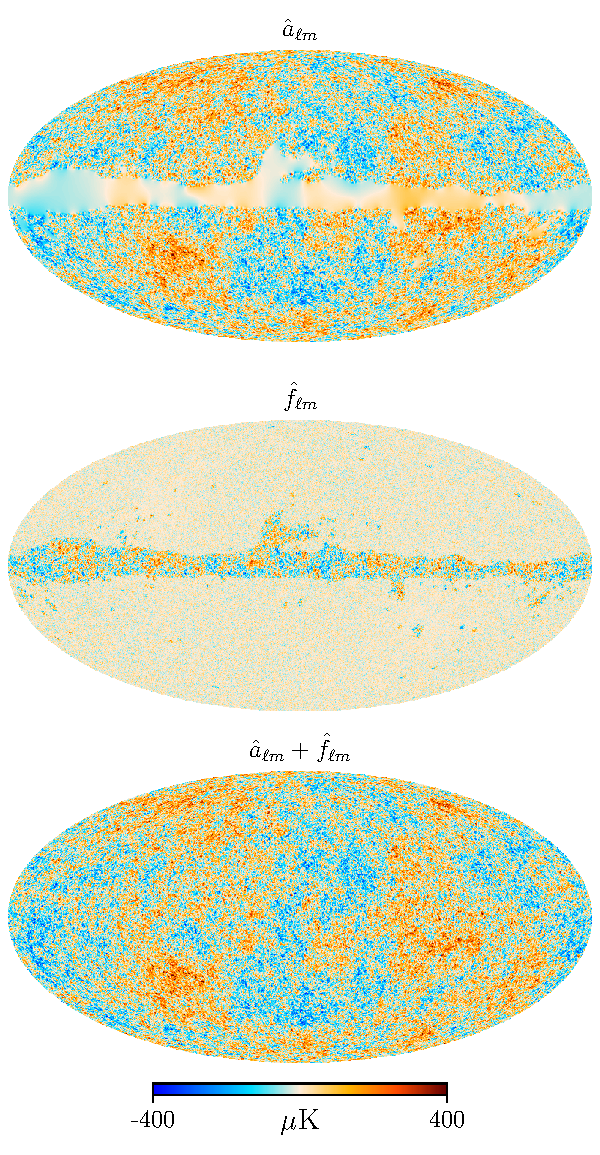
\includegraphics[width=\linewidth]{figures/s_hat_f_hat.pdf}
	\caption{\label{fig:sky_map}A constrained realization of a simulated CMB with a Galactic and point-source mask is decomposed into the mean field map $\hat{s}_{\ell m}$ and the fluctuation map $\hat{f}_{\ell m}$. The bottom panels shows the full sky map of the sample, $s_{\ell m} = \hat{s}_{\ell m} + \hat{f}_{\ell m}$.}
\end{figure}
\begin{figure}
	\centering
	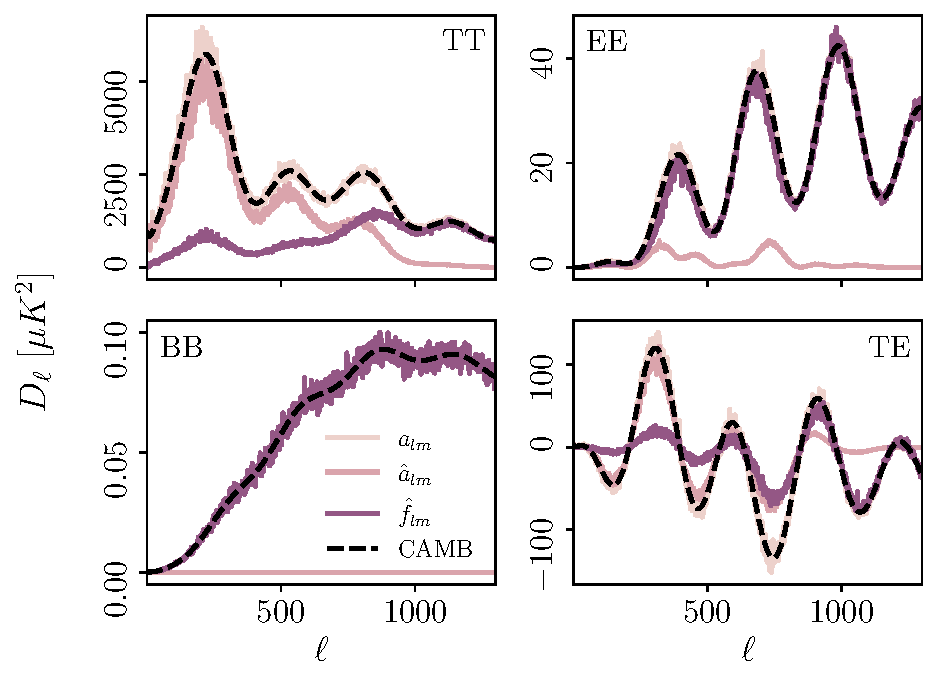
\includegraphics[width=\linewidth]{figures/sigma_ell.pdf}
	\caption{\label{fig:sigma_ell}The power spectra for the sky maps in Fig.~\ref{fig:sky_map}. This is compared to the $\Lambda$CDM power spectra used to generate the data.}
\end{figure}

In a setup with uniform noise on fullsky temperature data, this can be solved exactly in spherical harmonics space:
\begin{align}
    \label{eq:hat_s_approx}
    \hat{s}_{\ell m} &= d_{\ell m}\frac{A_{\ell}C_{\ell}}{N_\ell + A_{\ell}^2C_{\ell}},\\
    \label{eq:hat_f_approx}
    \hat{f}_{\ell m} &= w_{0\ell m}\frac{N_{\ell}\sqrt{C_{\ell}}}{N_\ell + A_{\ell}^2C_{\ell}}+w_{1\ell m}\frac{\sqrt{N_{\ell}}A_{\ell}C_\ell}{N_\ell + A_{\ell}^2C_{\ell}}.
\end{align}
In a more realistic scenario with non-uniform noise and masking, Eq.~\eqref{eq:mapmakingeq} becomes a computationally hard equation to solve. In \commanderthree, it is solved by the method of Conjugant Gradient which is the most time consuming part of the sampling process. In Appendix A, we show how this equation can be simplified for a constant latitude mask with isotropic noise. We made a Python script that does this calculation to verify our algorithm implementation in \commanderthree.

We visualize a constrained realization generated in \commanderthree\ in Fig.~\ref{fig:sky_map}. Here, we use a realistic Galactic plane and point-source mask and non-uniform noise. This configuration corresponds to the realistic setup we will discuss later in Sec.~\ref{sec:results}. Equations \eqref{eq:hat_s_approx} and \eqref{eq:hat_f_approx} are not valid due to $\boldsymbol{N}$ being non-diagonal in spherical harmonics space, and we need to solve the dense matrix equations in Eqs.~\ref{eq:mean-field-map} and \ref{eq:fluc-map}. The top panel shows the mean field map $\hat{s}_{\ell m}$. As the mask hides everything in the Galactic plane, we only have knowledge of large scale fluctuations inside the masked regions from the information outside of the mask. However, we lack knowledge of smaller scales in the masked regions, yielding a strong signal in the stocastic fluctuation map $\hat{f}_{\ell m}$. At even smaller scales outside of the masked regions, noise dominates and the uncertainty from noise is shown at very high multipoles in $\hat{f}_{\ell m}$. Putting both maps together gives us the sky map of this sample, $s_{\ell m} = \hat{s}_{\ell m} + \hat{f}_{\ell m}$.

We show the temperature and polarization power spectra of this sky map in Fig.~\ref{fig:sigma_ell}. At lower multipoles there is a high signal-to-noise (except for $BB$) and the mean field map $\hat{s}_{\ell m}$ dominates. But as we go to higher multipoles, noise starts dominating and all power comes from the fluctuation field $\hat{f}_{\ell m}$.

The second step of the Gibbs sampling in Eq.~\eqref{eq:theta-gibbs} can be sampled by an inverse Wishart ditribution, but we will not be using this step further in this work.

\begin{figure}
	\centering
	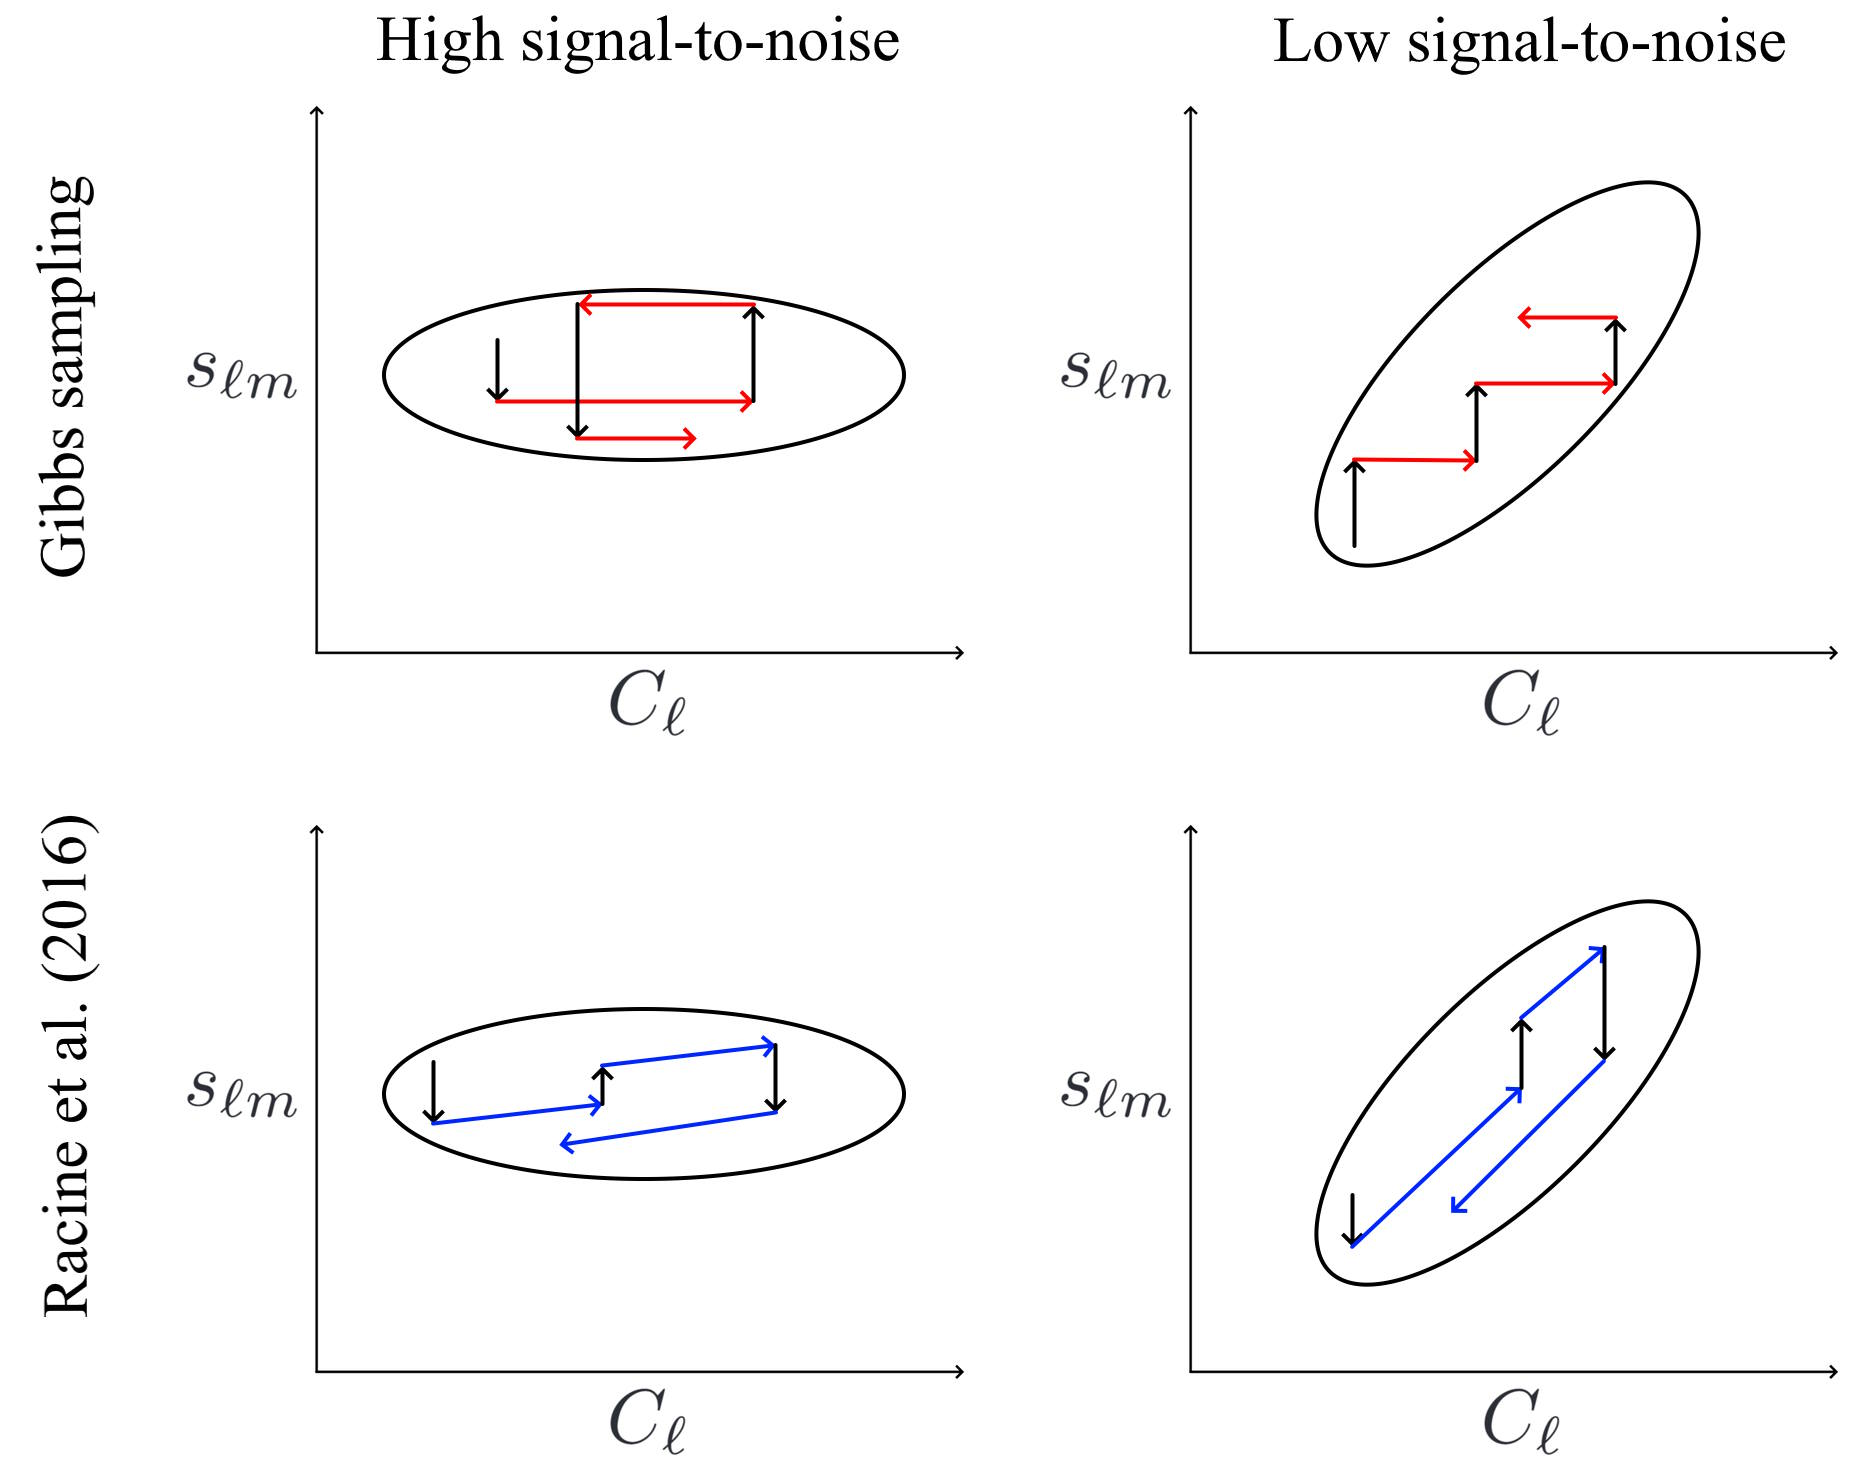
\includegraphics[width=\linewidth]{figures/parameter-estimation.jpg}
	\caption{\label{fig:illustration}Illustration of consequetive samples of the Gibbs sampler and the method of \cite{racine:2016}. The Gibbs sampler perform poorly in the low signal-to-noise regime as it requires a much larger number of samples to explore the posterior distribution as compared to the high signal-to-noise region. The joint sampler in the lower panels performs well in both regimes as it allows the next sample to move diagonally in parameter space as we sample $\boldsymbol{\theta}$, yielding $C_\ell(\boldsymbol{\theta})$ in the figure.}
\end{figure}

The Gibbs sampling method works well in high signal-to-noise regions, but performs poorly in the opposite limit. This can be understood by Eq.~\eqref{eq:fluc-map} when we have high instrumental noise, $\boldsymbol{N} \rightarrow \infty$, then we have no information of $s_{\ell m}$ from the data $d_{\ell m}$, and the sky map becomes only a realization of the variance $C_{\ell}$, i.e. $s_{\ell m} \rightarrow \hat{f}_{\ell m} = \sqrt{C_{\ell}} w_{0\ell m}$. Since we have no information of the mean field map $\hat{s}_{\ell m} \rightarrow 0$, we also do not know $C_\ell$. Hence, we get a strong degeneracy between the $C_\ell$ and $s_{\ell m}$. Gibbs sampling is well-known of performing poorly for strongly correlated parameters as you can not move diagonally in parameter space from one end of the joint posterior distribution to the other. This problem is shown in the top panel of Fig.~\ref{fig:illustration}, which shows the difference in the correlation length of Gibbs sampling between high and low signal-to-noise limits.

\subsection{Joint sampling}
\label{sec:joint-sampling}
A solution to the poor correlation length of the Gibbs sampling in low signal-to-noise regions was proposed by \cite{jewell:2009} further developed in \cite{racine:2016}. The authors suggested a Metropolis-Hasting sampler with a general proposal rule for $\theta$ and a rescaling of the fluctutation term of the sky signal. This allows the sampler to move diagonally in parameter space and more efficiently explore the full joint posterior distribution, as depicted in Fig.~\ref{fig:illustration}.

More precisely, one would perform
\begin{align}
    \boldsymbol{\theta}^{i+1} 
 &\leftarrow w(\boldsymbol{\theta} |\boldsymbol{\theta}^i)\\
 \boldsymbol{s}^{i+1} &\leftarrow P(\boldsymbol{s} | \boldsymbol{\theta}^{i+1}, \boldsymbol{d}),
\end{align}
for each Gibbs iteration, where the arrow denotes drawing a sample from the distribution on the right-hand side. $w(\theta |\theta^i)$ is the proposal distribution of the cosmological parameters. We use a multivariate Gaussian function,
\begin{equation}
w(\boldsymbol{\theta} |\boldsymbol{\theta}^i) = e^{-\frac12 \left(\boldsymbol{\theta} - \boldsymbol{\theta}^i \right)^T \boldsymbol{C}_{\boldsymbol{\theta}}^{-1}\left(\boldsymbol{\theta} - \boldsymbol{\theta}^i \right)}.
\end{equation}
For optimal chain convergence, the proposal variance $\boldsymbol{C}_{\boldsymbol{\theta}}$ should resemble the posterior distribution. The proposal variance we use is created from the samples of an earlier chain created with a diagonal proposal matrix.

They key altercation is to rescale the fluctuation map of the last accepted sample,
\begin{equation}
    \hat{f}_{\ell m}^{\textrm{scaled},\, i+1} = \left(\boldsymbol{C}^{i+1}_{\ell}\right)^{1/2}\left(\boldsymbol{C}^{i}_{\ell}\right)^{-1/2} \hat{f}_{\ell m}^{i},
\end{equation}
so that the map of sample $i+1$ is
\begin{equation}
    s_{\ell m}^{i+1} = \hat{s}_{\ell m}^{i+1} + \left(\boldsymbol{C}^{i+1}_{\ell}\right)^{1/2}\left(\boldsymbol{C}^{i}_{\ell}\right)^{-1/2} \hat{f}_{\ell m}^{i}.
\end{equation}
In low signal-to-noise regions, this rescaling allows diagonal moves in $s_{\ell m} - C_\ell$ space of Fig.~\ref{fig:illustration}. The acceptance rate for this proposal was calculated in \cite{racine:2016} to be
\begin{equation}
    \label{eq:acceptance-rate}
    A = \mathrm{min}\left[1, \frac{\pi(\boldsymbol{\theta}^{i+1})}{\pi(\boldsymbol{\theta}^i)} \frac{w(\boldsymbol{\theta}^{i} |\boldsymbol{\theta}^{i+1})}{w(\boldsymbol{\theta}^{i+1} |\boldsymbol{\theta}^i) }\frac{P(\boldsymbol{\theta}^{i+1})}{P(\boldsymbol{\theta}^i)} \right].
\end{equation}
Here, $P(\boldsymbol{\theta})$ is the prior on $\boldsymbol{\theta}$ and
\begin{align}
    \nonumber
    \pi(\boldsymbol{\theta}^{i}) = \mathrm{exp}\bigg[&-\frac12 \left(\boldsymbol{d}-\boldsymbol{A}\boldsymbol{\hat{s}}^i\right)^T \boldsymbol{N}^{-1}\left(\boldsymbol{d}-\boldsymbol{A}\boldsymbol{\hat{s}}^i\right)\\
    &-\frac12\boldsymbol{\hat{s}}^{i,T} \boldsymbol{S}^{i, -1}\boldsymbol{\hat{s}}^i -\frac12 \boldsymbol{\hat{f}}^{i, T}\boldsymbol{A}^T\boldsymbol{N}^{-1} \boldsymbol{A}\boldsymbol{\hat{f}}^i\bigg],
\end{align}
where we have omitted the $\theta^i$ dependence of $\hat{s}^i$, $\hat{f}^i$ and $S^i$. Our proposal matrix for the cosmological parameters is symmetric, $w(\boldsymbol{\theta}^{i} |\boldsymbol{\theta}^{i+1}) = w(\boldsymbol{\theta}^{i+1} |\boldsymbol{\theta}^{i})$, and hence we can remove them from Eq.~\eqref{eq:acceptance-rate}.

We note that the acceptance rate will use the scaled fluctuation term, $f_{\ell m}^{\textrm{scaled}, i+1}$, for sample $i+1$ instead of the calculated fluctuation term in Eq.~\eqref{eq:mapmakingeq}. Hence, we only need to calculate $f_{\ell m}^{i+1}$ from this equation if the sample is accepted. This allows us to save roughly half the computational time of discarded samples as compared to accepted samples.

The algorithm can be broken down into these steps:
\begin{enumerate}
    \item Start with an initial value $\boldsymbol{\theta}^0$. From that, calculate the power spectra $\boldsymbol{S}^0$, the mean-field map $\boldsymbol{\hat{s}}^0$ and the fluctuation map $\boldsymbol{\hat{f}}^0$ from the cosmological parameters.
    \item Pick a new cosmological parameter sample, $\boldsymbol{\theta}^{i+1}$. Calculate $\boldsymbol{S}^{i+1}$, $\boldsymbol{\hat{s}}^{i+1}$ and the \textit{scaled} fluctuation term $f_{\ell m}^{\textrm{scaled}, i+1}$.
    \item Calculate the acceptance term of Eq.~\ref{eq:acceptance-rate}, and accept/reject according to the regular Metropolis-Hasting rule.
    \item If the sample is accepted, then calculate $f_{\ell m}^{i+1}$. This term will in the next iteration become $f_{\ell m}^{i}$ which will appear in the acceptance probability and the equation for $f_{\ell m}^{\textrm{scaled}, i+1}$. The fluctuation map is not necessary to calculate if the sample is discarded.
    \item Iterate 2-4.
\end{enumerate}

\begin{figure}
	\centering
	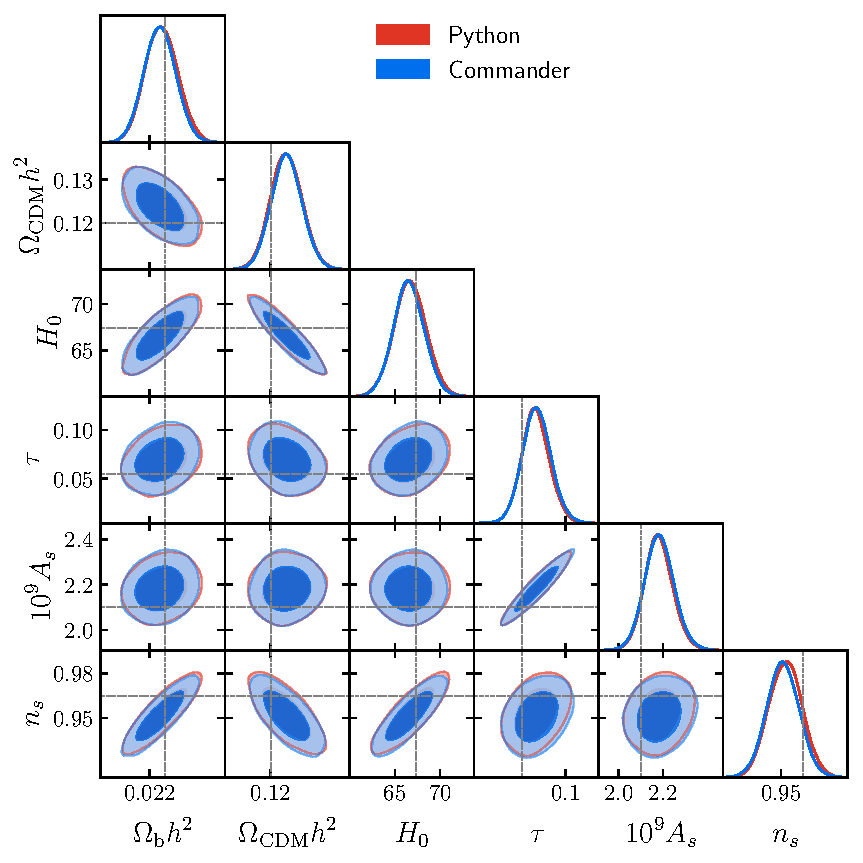
\includegraphics[width=\linewidth]{figures/dist_posterior_no_mask.pdf}
	\caption{\label{fig:nomask}Parameter estimation on a CMB realization with isotropic noise. We use $N_{\mathrm{side}}=512$ and the beam convolve using the beam window functions of 70\,GHz band of Planck. No mask is applied.}
\end{figure}

In this work, we sample the 6 $\Lambda$CDM parameters, i.e. $\boldsymbol{\theta}=(\Omega_{\textrm{b}}h^2, \Omega_{\textrm{CDM}}h^2, H_0, \tau, A_s, n_s)$. Here, $\Omega_\mathrm{b}$ and $\Omega_\mathrm{CDM}$ are the current density of baryonic and cold dark matter, respectively. $H_0$ si the Hubble constant today, while $h$ is the normalized Hubble constant, $h=\frac{H_0}{100\,\mathrm{km s}^{-1} \mathrm{MPc}^{-1}}$. $\tau$ is the optical depth at reionization, $A_s$ is the amplitude and $n_s$ is the tilt of the scalar primordial power spectrum. We use \texttt{CAMB}\footnote{\url{https://github.com/cmbant/CAMB}} to generate the $\Lambda$CDM power spectra $\boldsymbol{C}_{\ell}(\boldsymbol{\theta})$ \citep{Lewis:1999bs}.


\section{Results}
\label{sec:results}

We implement the algorithm into the \commanderthree\ framework with the aim of being a part of the full Gibbs sampling chain alongside sampling of instrumental and astrophysical parameter in future work.

To verify the implementation, we also created a special-prupose Python script that samples cosmological parameters on a CMB simulation with uniform noise and a constant latitude mask. We show how we calculate an analytic expression for $N^{-1}_{\ell m \ell' m'}$ in Appendix A, and how that simplifies matrix equations such as the map making equation and acceptance rate. This Python script has been made publically available\footnote{\url{https://github.com/LilleJohs/}}. We also use Cobaya \citep{Torrado:2020dgo} to verify uniform noise on full sky data.

We create two sets of CMB simulations: One with uniform noise and one with non-uniform noise using a realization of a randomly picked RMS noise map of the 70\,GHz from the official BeyondPlanck chain. Both simulations are created using $N_{\textrm{side}}=512$ and the public Planck Data Release 4 70\,GHz beams \citep{npipe}.

First, we run the uniform noise simulation without a mask in Cobaya, Python and \commanderthree\ to make sure the three implementations agree with each other. This case can be solved exactly using the likelihood presented in Section \ref{sec:exact-likelihood} which we do using Cobaya \citep{Torrado:2020dgo}, while the Python script implements the method of \citet{racine:2016}. Fig.~\ref{fig:nomask} shows the posterior distribution of the cosmological parameters from 50 000 samples each of \commanderthree, Python and Cobaya, and we find excellent agreement between the three implementations.

\begin{figure}
	\centering
	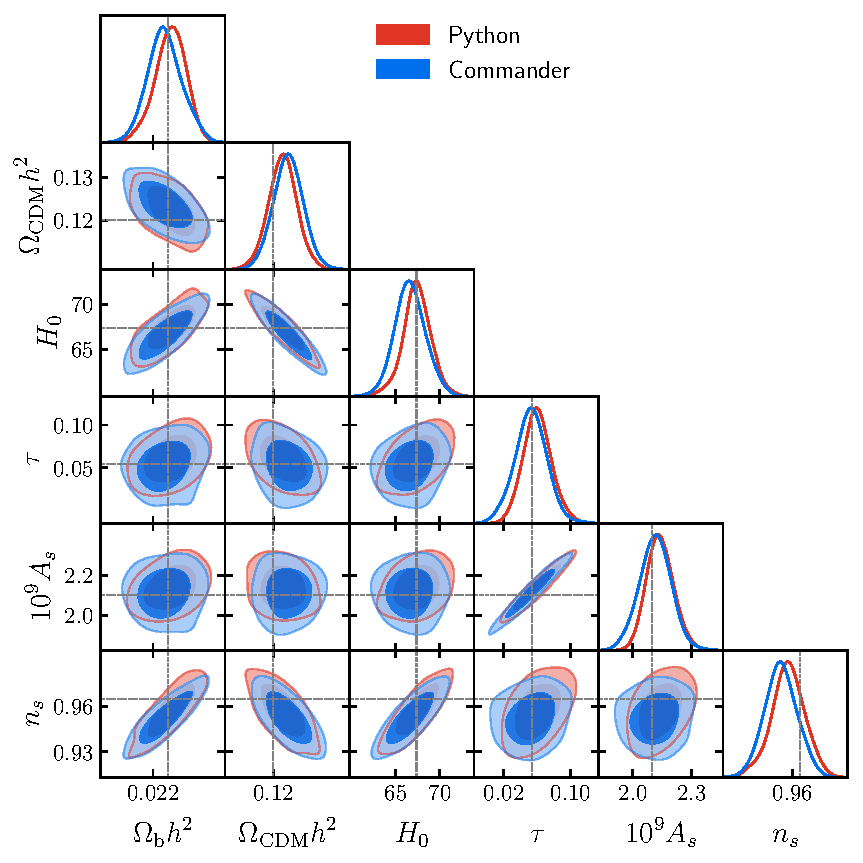
\includegraphics[width=\linewidth]{figures/dist_posterior_10_mask.pdf}
	\caption{\label{fig:mask10}Cosmological parameter estimation on same simulation as in Fig.~\ref{fig:nomask} but a constant latitude mask is applied so that the sky fraction is 90\%.}
\end{figure}

We then proceed by adding a constant latitude mask of latitude $\arcsin(0.1) \sim 5.7^\circ$ as this gives the sky coverage $f_{\mathrm{sky}} = 0.90$. $\boldsymbol{N}$ is no longer diagonal and the brute-force method of Section \ref{sec:exact-likelihood} will be computationally intractable. 

We use the Python implementation for this case, but we note that it is computationally demanding with a single accepted sample taking 853 CPU-hours. Note, that an accepted sample takes longer to calculate than a discarded sample as we only calculate the fluctuation map $f^i_{\ell m}$ if sample $i$ is accepted.

We show the posterior distribution of $\sim 5000$ Python samples and $\sim 9000$ \commanderthree\ samples in Fig.~\ref{fig:mask10}. Although we have a lack of independent samples due to the long correlation length and computational cost, we find good an agreement between the two implementations.

\begin{figure}
	\centering
	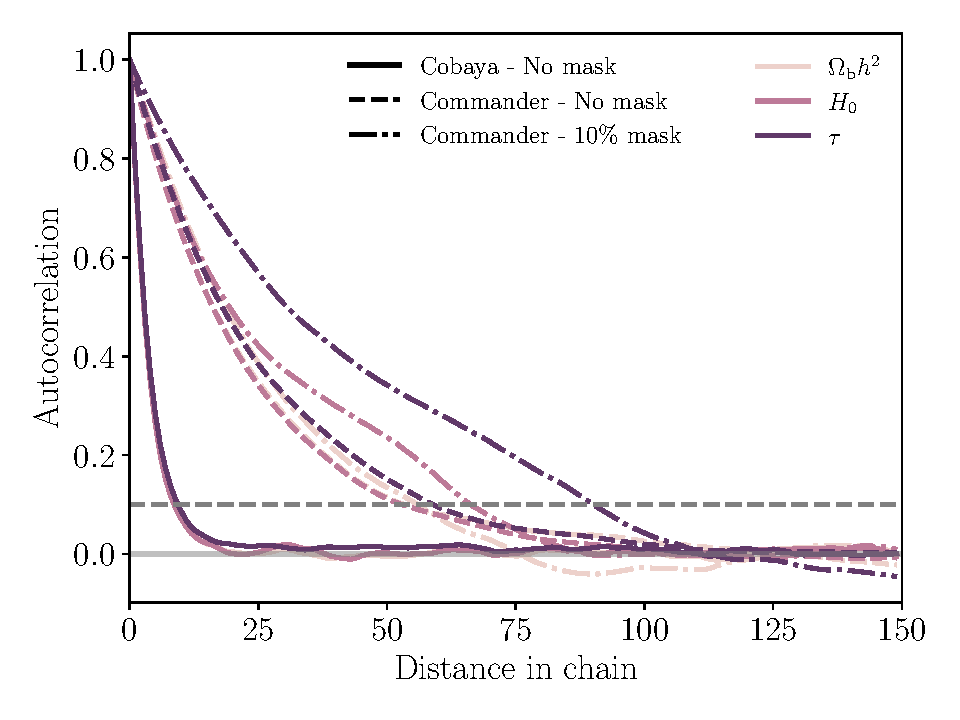
\includegraphics[width=\linewidth]{figures/auto_correlation.pdf}
	\caption{\label{fig:autocorrelation}Auto correlations of some cosmological parameters.}
\end{figure}

We calculate the autocorrelation function for three cosmological parameters for three chains in Fig.~\ref{fig:autocorrelation}. We show the brute-force likelihood method in Cobaya which has a correlation length $\lesssim 10$. Cosmological parameter sampling using the likelihood-free estimator in \commanderthree\ for the same case is also shown and exhibits a correlation length 5 times higher than the brute-force likelihood.

Although we are sampling the same simulated CMB map without a mask in \commanderthree\ and Cobaya, we expect a higher correlation length as the algorithm of \citet{racine:2016}  the sky signal $s_{\ell m}$. We also show in addition the case with a $10\%$ mask, which increases the correlation length as compared to full-sky.

\subsection{Realistic mask and noise}

\begin{figure}
	\centering
	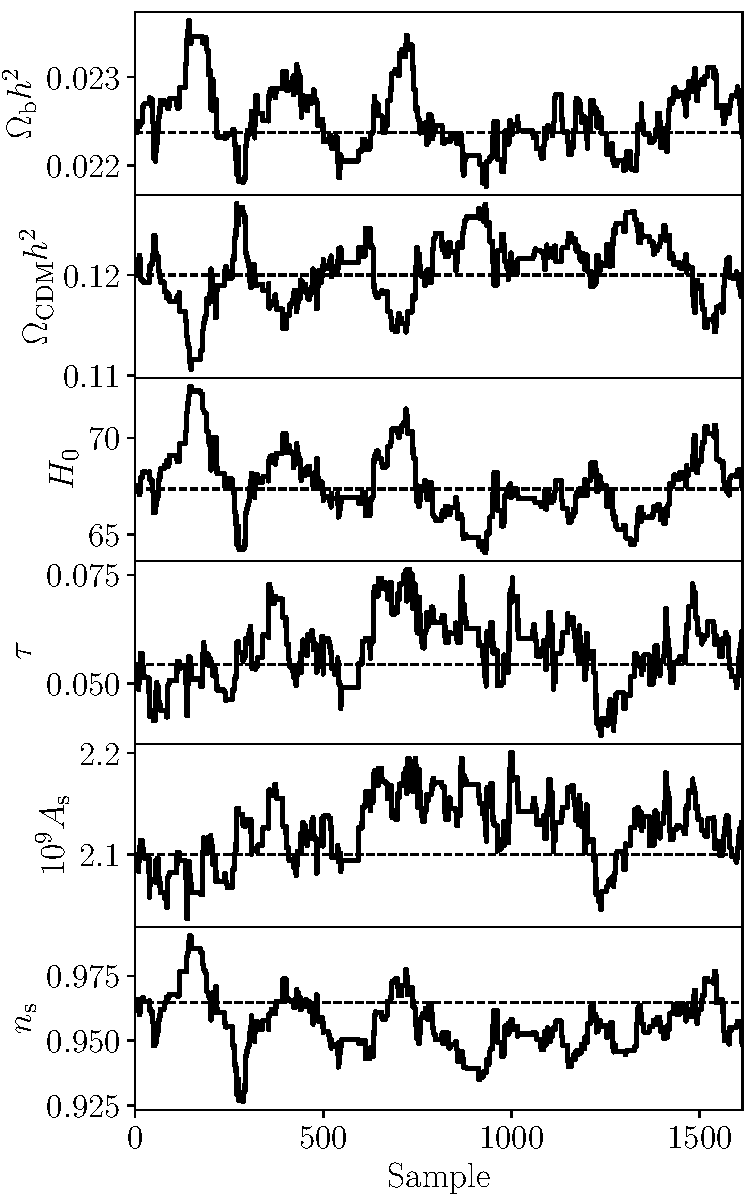
\includegraphics[width=\linewidth]{figures/realistic_chain.pdf}
	\caption{\label{fig:traceplot}Traceplot of the cosmological parameters for the $70\,$GHz case. The dashed lines show the input value of the CMB simulation.}
\end{figure}

We then turn to a more realistic case: We make a realization of a 70\,GHz noise map and a realistic Galactic and point source mask of $f_{\mathrm{sky}}=0.85$. Our Python implementation can not sample this case as it neither supports anisotropic noise nor a realistic mask. Hence, we can only rely on the CG iterator of \commanderthree3.

In Fig.~\ref{fig:traceplot} we show the traceplots of the cosmological parameters from this run. We did not include this chain into the autocorrelation Fig.~\ref{fig:autocorrelation} as we have few samples for it converge, but it is clear by eye that the correlation length is $\mathcal{O}(100)$.

\begin{figure}
	\centering
	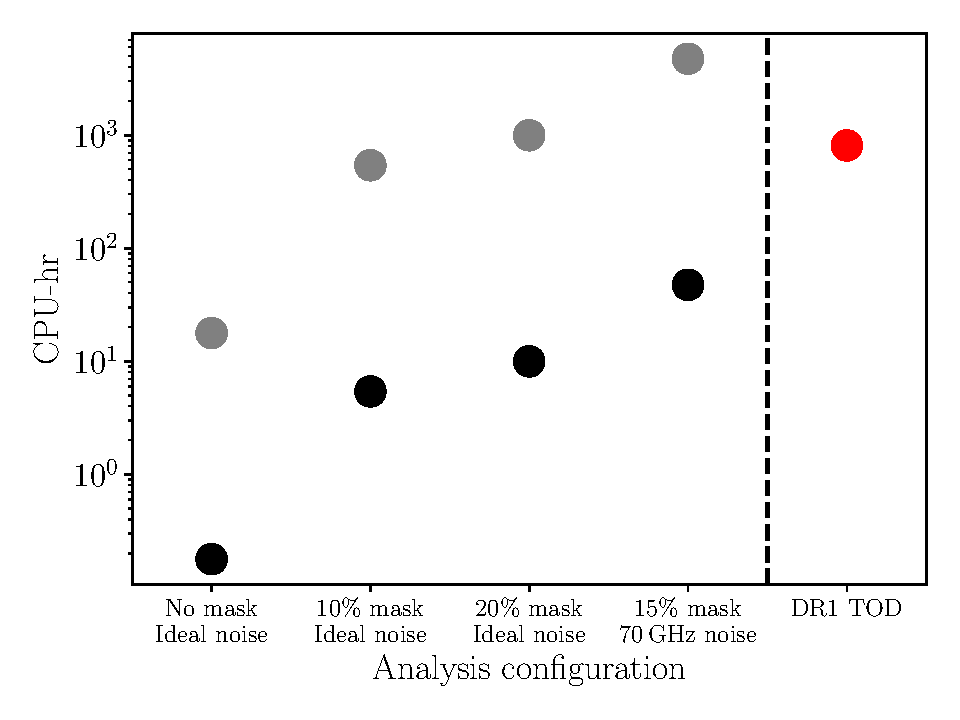
\includegraphics[width=\linewidth]{figures/run_time.pdf}
	\caption{\label{fig:runtime}CPU-hours per accepted sample. This is compared to the 812 CPU-hours to generate one single end-to-end sample of \planck\ LFI and \wmap\ channels in red.}
\end{figure}

We are limit by a lack of independent samples due to the large correlation length and a very high cost computational cost of one sample. We show the current CPU-hour per accepted joint sample in Fig.~\ref{fig:runtime} for the different configuration. These cases are compared to the 812 CPU-hours it takes to generate one Cosmoglobe DR1 Gibbs sample from TOD in red. This shows that more works need to be done to lower the computational time to generate a joint sample, as we want to include the methods into the Cosmoglobe framework on actual data.

The computational time is dominated by solving Eq.~\eqref{eq:mapmakingeq} by the method of Conjugant Gradient (CG). For the 70\,GHz case, we currently require 5000 CG iterations to generate one sample of the CMB which takes 46 CPU-hours. With a correlation length of $\sim 100$ samples, we then find 4600 CPU-hours to generate an individual sample of the cosmological parameters. Hence, work is needed to lower the computational cost of solving Eq.~\eqref{eq:mapmakingeq} as we do not see a way to shorten the correlation length of the algortihm.

Lowering this number can be done by better preconditioning and Hamiltonian sampling and blablabla \textcolor{red}{This part is for HK}

\section{Conclusions}
\label{sec:conclusions}

We have shown that the algorithm presented in \cite{racine:2016} works well in the \commanderthree framework for anisotropic noise and mask.

\bibliographystyle{../common/aa}

\bibliography{../common/Planck_bib,../common/CG_bibliography}

\appendix

\section{Analytic expression for a constant latitude mask}
\label{sec:appendixA}


The goal of this appendix is to show how we can calculate $N_{\ell m \ell' m'}^{-1}$ analytically for a constant latitude mask and uniform noise, and how this expression makes the map making equation computationally fast to solve. The noise can be written as this in pixel space:
$$
\left(N^{-1} \right)_{pp'} = \frac{N_{\mathrm{pix}}}{\sigma^2} \delta_{pp'} H(|\theta(p) -\pi/2|-b).
$$
where $H$ is the Heavyside function, meaning that we mask every pixel $p$ where $|\theta(p) -\pi/2| < b$ for some latitude $b$ in radians. For a masked pixel, $\left(N^{-1} \right)_{pp}=0$ which means that $N_{pp} = \infty$ for that pixel, as we want.

Using that
$$
\left(N^{-1}\right)_{pp'} = \sum_{\ell m}\sum_{\ell' m'} \left(N^{-1}\right)_{\ell m \ell'm'} Y_{\ell m}\left(p\right)Y^*_{\ell' m'}\left(p'\right),
$$
where $Y_{\ell m}\left(p\right) = Y_{\ell m}\left(\hat{n}(p)\right)$ and $\hat{n}(p)$ are the spherical coordinates for pixel $p$, we can transform to spherical harmonics space,
\begin{align}
\nonumber
\left(N^{-1}\right)_{\ell m \ell' m'} &= \sum_{p p'}\left(N^{-1}\right)_{pp'}Y^{*}_{\ell m}(p)Y_{\ell' m'}(p')\\
\nonumber
&= \frac{N_{\mathrm{pix}}}{\sigma^2}\sum_{p p'} Y^{*}_{\ell m}(p)Y_{\ell' m'}(p') \delta_{pp'} H(|\theta -\pi/2|-b)\\
\nonumber
&= \frac{N_{\mathrm{pix}}}{\sigma^2}\sum_{p } Y^{*}_{\ell m}(p)Y_{\ell' m'}(p) H(|\theta -\pi/2|-b)\\
&= \frac{N_{\mathrm{pix}}}{\sigma^2}\sum_p \Tilde{Y}_{\ell m}\Tilde{Y}_{\ell' m'} e^{-i(m-m')\phi} H(|\theta -\pi/2|-b).
\end{align}
Here, we used that $Y_{\ell m}(p) = \tilde{Y}_{\ell m} e^{im\phi}$ where it is implied that $\tilde{Y}_{\ell m}=\tilde{Y}_{\ell m}(\theta)$, and $\theta$ and $\phi$ are functions of $p$.

We now take the limit where there is a large amount of pixels with equal surface area each. In this limit, we change the sum into an integration where we account for the number of pixels per area element
\begin{equation}
\sum_p \rightarrow \frac{N_{\mathrm{pix}}}{4\pi}\int d\Omega  = \frac{N_{\mathrm{pix}}}{4\pi}\int_{0}^{2\pi} d\phi \int_{0}^{\pi} d\theta \sin(\theta).
\end{equation}
This gives us in spherical coordinates
\begin{align}
\nonumber
\left(N^{-1}\right)_{\ell m \ell' m'} &= \frac{N_{\mathrm{pix}}^2}{4\pi \sigma^2}\int_{0}^{2\pi} d\phi \int_{0}^{\pi} d\theta \sin(\theta)\tilde{Y}_{\ell m}  \tilde{Y}_{\ell' m'}  e^{-i(m-m')\phi}
\\
\nonumber
&\cdot H(|\theta -\pi/2|-b)\\
\nonumber
&= \frac{N_{\mathrm{pix}}^2}{2\sigma^2} \delta_{mm'}\int_{0}^{\pi} d\theta \sin(\theta)\tilde{Y}_{\ell m}  \tilde{Y}_{\ell' m'} H(|\theta -\pi/2|-b)\\
\nonumber
&= \frac{N_{\mathrm{pix}}^2}{2\sigma^2} \delta_{mm'}\\
&\cdot \left(\int_{0}^{\pi/2-b} d\theta \sin(\theta) \tilde{Y}_{\ell m}  \tilde{Y}_{\ell' m'}+\int_{\pi/2+b}^{\pi} d\theta \sin(\theta)\tilde{Y}_{\ell m}  \tilde{Y}_{\ell' m'}\right).
\end{align}
Writing the above equation in terms of Legendre polynomials $P_{\ell m}(\cos(\theta)))$, we have
$\Tilde{Y}_{\ell m} = \Delta_{\ell m}P_{\ell m}(\cos(\theta)))$, where ${\Delta_{\ell m}=(-1)^m \sqrt{\frac{2\ell+1}{4\pi}\frac{(\ell - m)!}{(\ell+m)!}}}$.
 Writing $x=\cos(\theta)$, we know that Legendre polynomials $P_{\ell m}(x)$ are either symmetric or antisymmetric in $x\rightarrow-x$. $P_{\ell m}(x)$ is symmetric in $x \rightarrow -x$ when $\ell+m$ = even and antisymmetric when $\ell+m$ = odd. Since $m=m'$, we note that the two integrals cancel each other if $\ell+\ell' =$ odd. We, therefore, only get non-zero elements when $\ell + \ell' =$ even, for which the two integrals are equal. Hence, for $\ell + \ell'=$ even, we get
\begin{align}
\nonumber
\left(N^{-1}\right)_{\ell m \ell' m'} &= \frac{N_{\mathrm{pix}}^2}{\sigma^2} \delta_{mm'}\int_{0}^{\pi/2-b} d\theta \sin(\theta)\Tilde{Y}_{\ell m}(\theta)\Tilde{Y}_{\ell' m'}(\theta)\\
\label{eq:finished_n_inv}
&=\frac{N_{\mathrm{pix}}^2}{\sigma^2} \delta_{mm'}\int_{\sin(b)}^{1} dx \, \Tilde{Y}_{\ell m}(\arccos(x)) \Tilde{Y}_{\ell' m}(\arccos(x)).
\end{align}
This integral can be solved numerically by gridding $x$, and the spherical harmonics where the phase factor is removed can be calculated in Python using a library like ...

The azimutally symmetric Galactic mask used for this work has a sky coverage of $f_{\mathrm{sky}} = 0.90$, giving $\sin(b) = 0.1$. Therefore, we require much fewer grid points for $x$ if we use the following identity for $\ell+\ell' = $ even:
\begin{align}
&\delta_{mm'} \int_{\sin(b)}^{1} dx \, \Tilde{Y}_{\ell m}(\arccos(x)) \Tilde{Y}_{\ell' m}(\arccos(x)) = \\
\frac{1}{4\pi}\delta_{\ell \ell'}\delta_{m m'} - &\delta_{mm'} \int_{0}^{\sin(b)} dx \, \Tilde{Y}_{\ell m}(\arccos(x)) \Tilde{Y}_{\ell' m}(\arccos(x)),
\end{align}
which comes from the orthonormality condition for spherical harmonics. We now only need to grid $x$ in the interval $0\leq x \leq \sin(b) = 0.1$, as opposed to the interval $0.9 \leq x \leq 1$.

Since $N^{-1}_{\ell m \ell' m'} \propto \delta_{m m'}$, we get simplified matrix expressions. Imagine multiplying the matrix $\boldsymbol{N}^{-1} = N^{-1}_{\ell m \ell' m'}$ with the vector $\boldsymbol{b} = b_{\ell m}$
\begin{align}
\boldsymbol{N}^{-1} \cdot \boldsymbol{b} &= \sum_{\ell' m'}\left(N^{-1}\right)_{\ell m \ell' m'}b_{\ell' m'} = \sum_{\ell'}\left(N^{-1}\right)_{\ell m \ell' m}b_{\ell' m}\\
&= \sum_{\ell' }\left(N^{-1}\right)^{(m)}_{\ell, \ell'}b^{(m)}_{\ell'}.
\end{align}
To solve the map-making equation, we get a matrix equation for each $0 \leq m \leq \ell_{\mathrm{max}}$. This gives us $\ell_{\textrm{max}}+1$ number of matrix equations where the dimensions of the matrices are maximally $\ell_{\textrm{max}} \times \ell_{\textrm{max}}$. This is numerically much quicker than inverting the full $(\ell_{\textrm{max}})^2 \times (\ell_{\textrm{max}})^2$ matrix once.


\end{document}
